% Figure 2: three crops of the session page (recorded Pokec session, the turn with two readings), with callouts.
% Build: tectonic fig2-session.tex, then move the PDF one level up.
\documentclass[border=0pt]{standalone}
\usepackage{graphicx}
\usepackage{tikz}
\newcommand{\crop}[4]{% name, x, file and options, width
  \node[anchor=north west, inner sep=0pt, draw=black!25, line width=0.3pt] (#1) at (#2,0) {\includegraphics[width=#4]{#3}};}
\newcommand{\callout}[4]{% image node, x fraction, y fraction, letter
  \path (#1.north west) -- (#1.north east) coordinate[pos=#2] (mx);
  \path (#1.north west) -- (#1.south west) coordinate[pos=#3] (my);
  \node[circle, fill=black!85, text=white, inner sep=0.9pt, font=\sffamily\bfseries\scriptsize, minimum size=3.6mm] at (mx |- my) {#4};}
\begin{document}
\begin{tikzpicture}
\crop{left}{0}{f2-left.png}{5.95cm}
\node[anchor=north west, inner sep=0pt, draw=black!25, line width=0.3pt] (card) at (6.2,0) {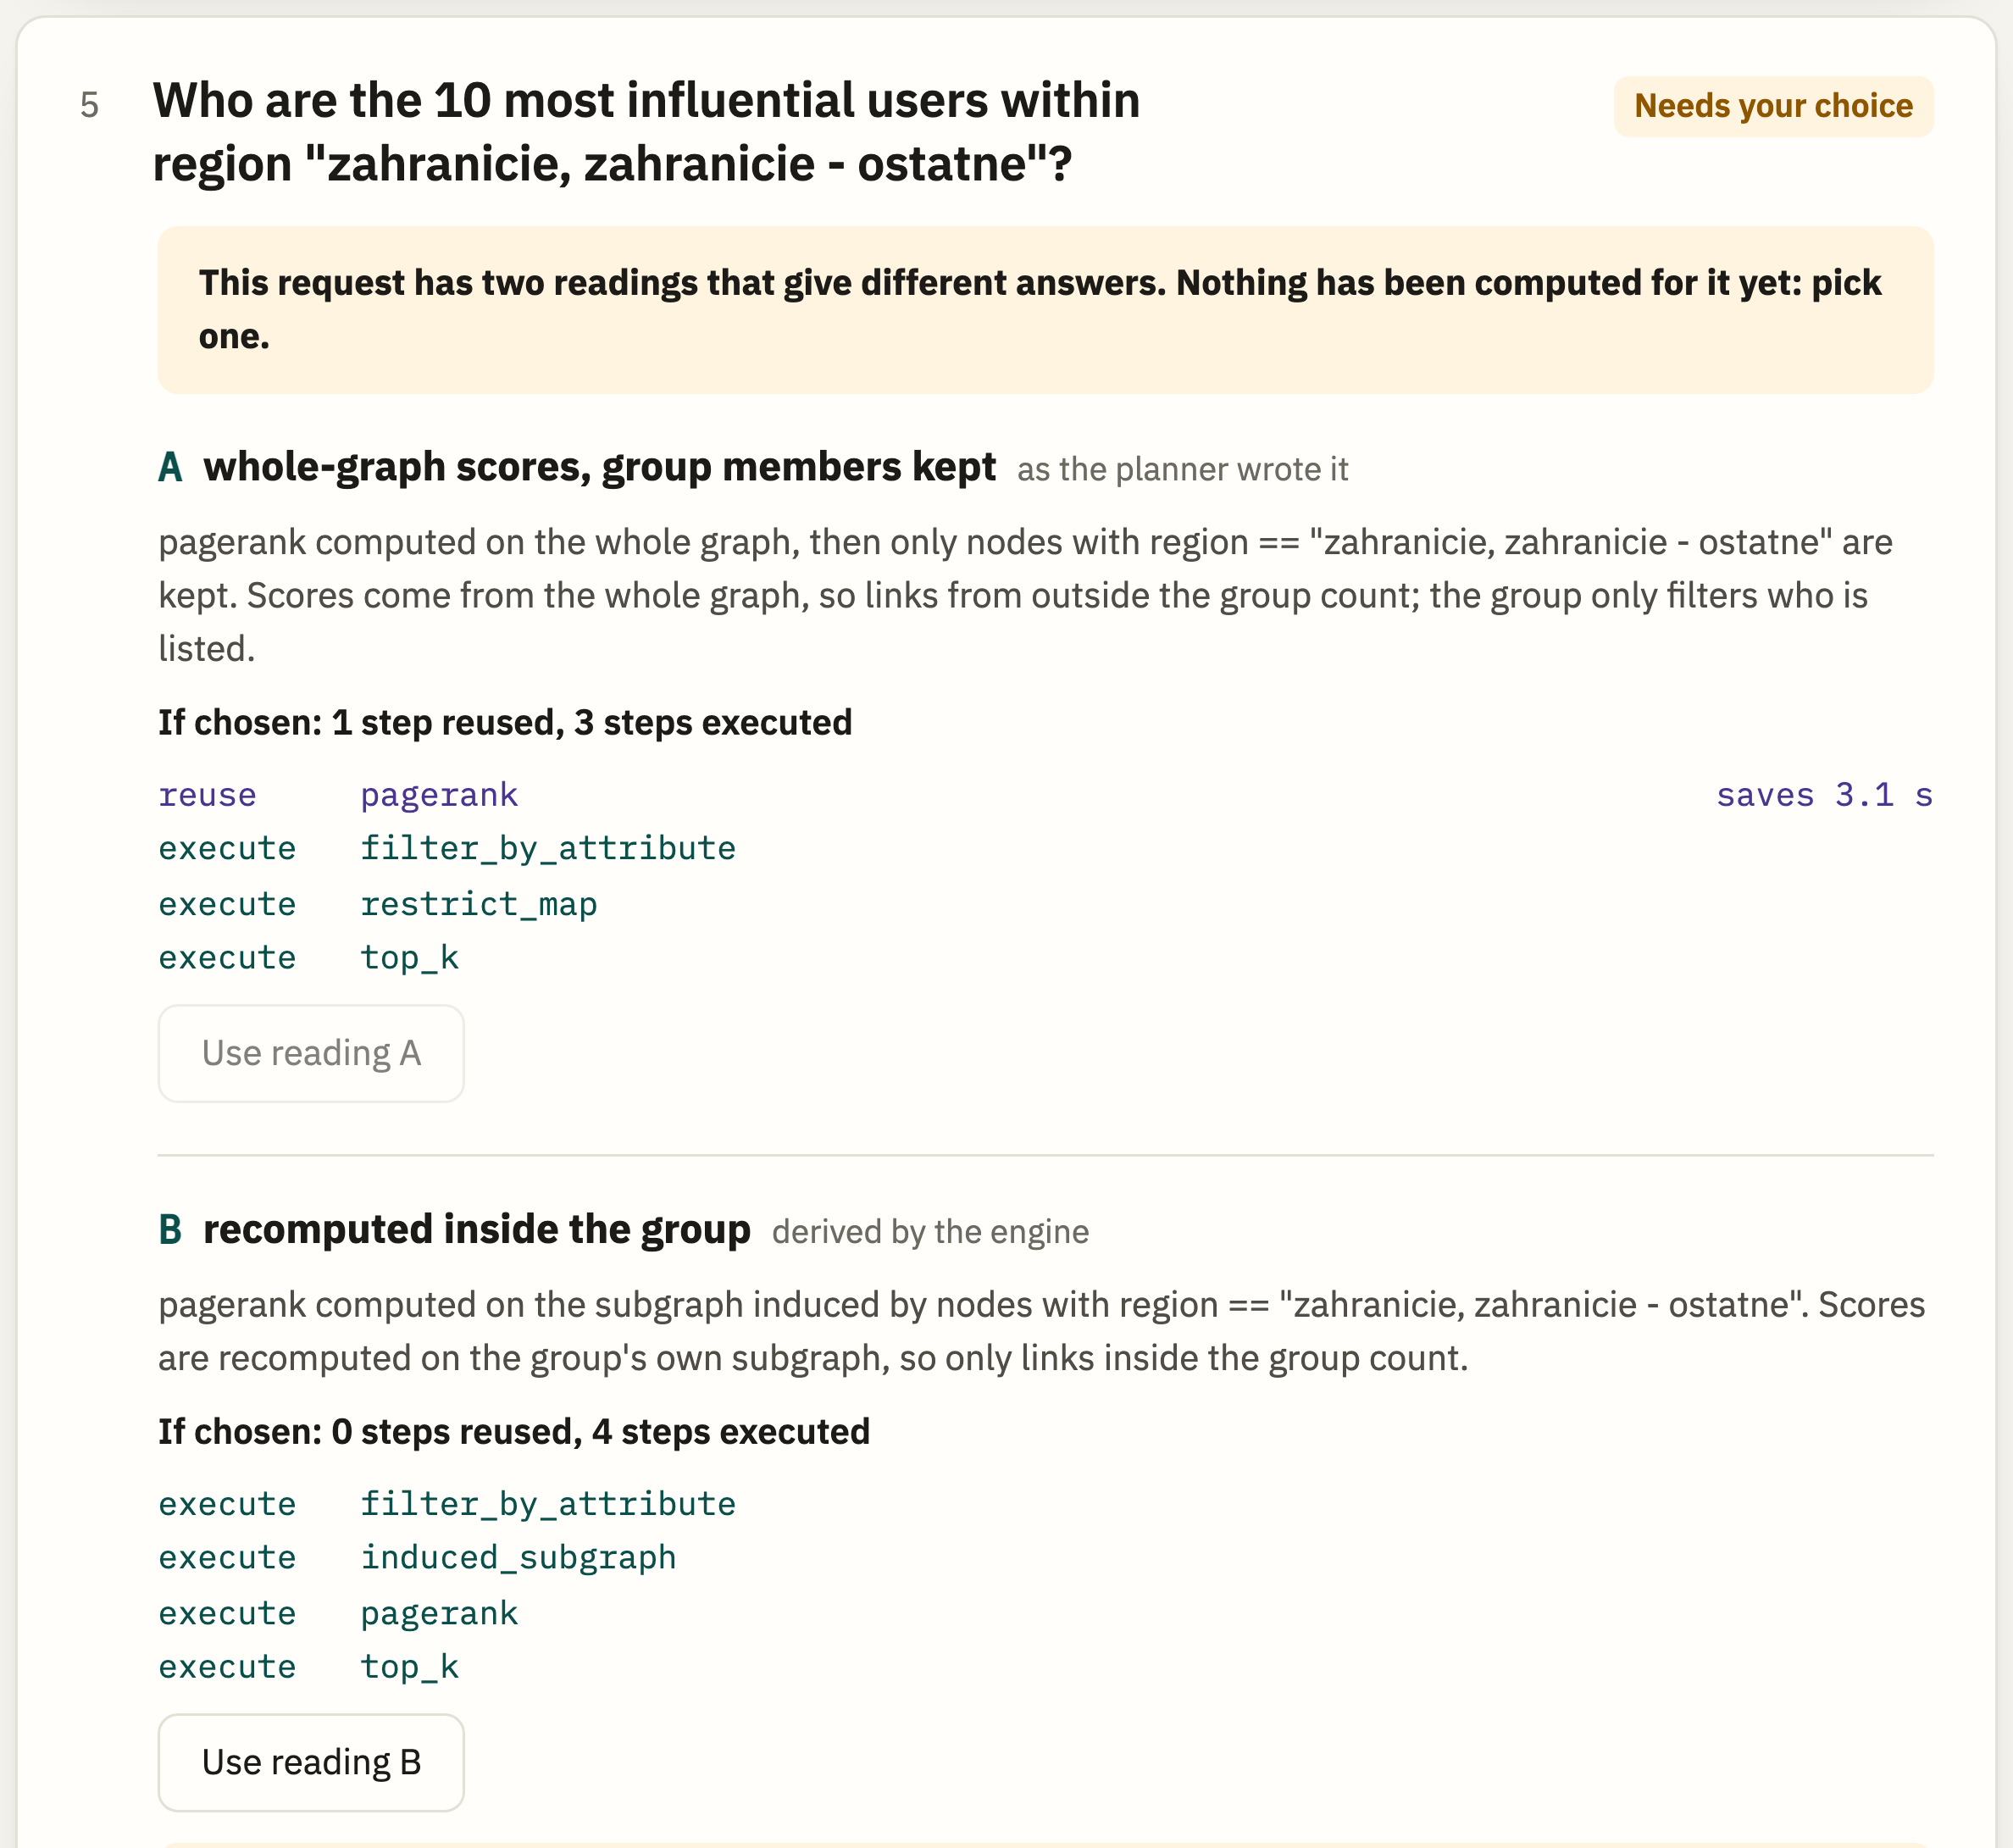
\includegraphics[width=7.97cm, trim=0 14 0 0, clip]{f2-card.png}};
\crop{ledger}{14.42}{f2-ledger.png}{3.18cm}
\callout{left}{0.755}{0.118}{a}
\callout{left}{0.945}{0.243}{b}
\callout{card}{0.755}{0.049}{c}
\callout{ledger}{0.90}{0.05}{d}
\end{tikzpicture}
\end{document}
